\section{Overview}

%1. What is an HPD
%2. What is its purpose
%3. Layout and dimensions
%4. Operation
%5. Performance
The Hybrid photon detectors (HPD) are used to detect Cherenkov photons emitted by particles traversing the RICH system. The hit positions of the emitted photons form a ring on the HPD plane, the radius of which is related to the Cherenkov angle associated to the particle. The Cherenkov angle of a particle acts as a signature of its particle type. This enables discrimination between electrons, pions, kaons and protons which is needed to identify the decay processes of particles produced in the LHCb detector. 

The HPDs are arrange in two grids, for RICH 1 [RICH 2] the grids are positioned above [left] and below [right] the beamline and are are arranged into rows of $14$ [$16$] by $7$ [$9$] columns (Fig \ref{fig: RICH 1: upper grid}). The HPDs are approximately cylindrical in shape, with a length of $160\,\mathrm{mm}$ and radius of $43.7\,\mathrm{mm}$ \footnote{There are small differences in the dimensions of the HPDs in RICH1 and RICH2. The values given here are for the HPDs in RICH 1, details for the HPDs in RICH 2 can be found in the RICH Technical design report.} (See Fig \ref{fig: HPD schematic} and Fig \ref{fig:HPD_photo}). A spherically-shaped cap quartz window is attached to one end of the HPD, on its inner surface is a deposition of an S20 (multi alkali) photo-cathode which emits photo-electrons when stimulated by photons. The emitted photo-electrons traverse the vacuum chamber of the HPD where they are accelerated by an electric potential difference of $20\,\mathrm{kV}$ onto a square silicon chip array of $32\,\times\,32$ pixels \footnote{When the HPD is run is its ALICE configuration the pixel dimensions are $32\,\times\,256$ pixels} with a length and width of $16\,\mathrm{mm}$.

\begin{figure}
	\begin{center}
		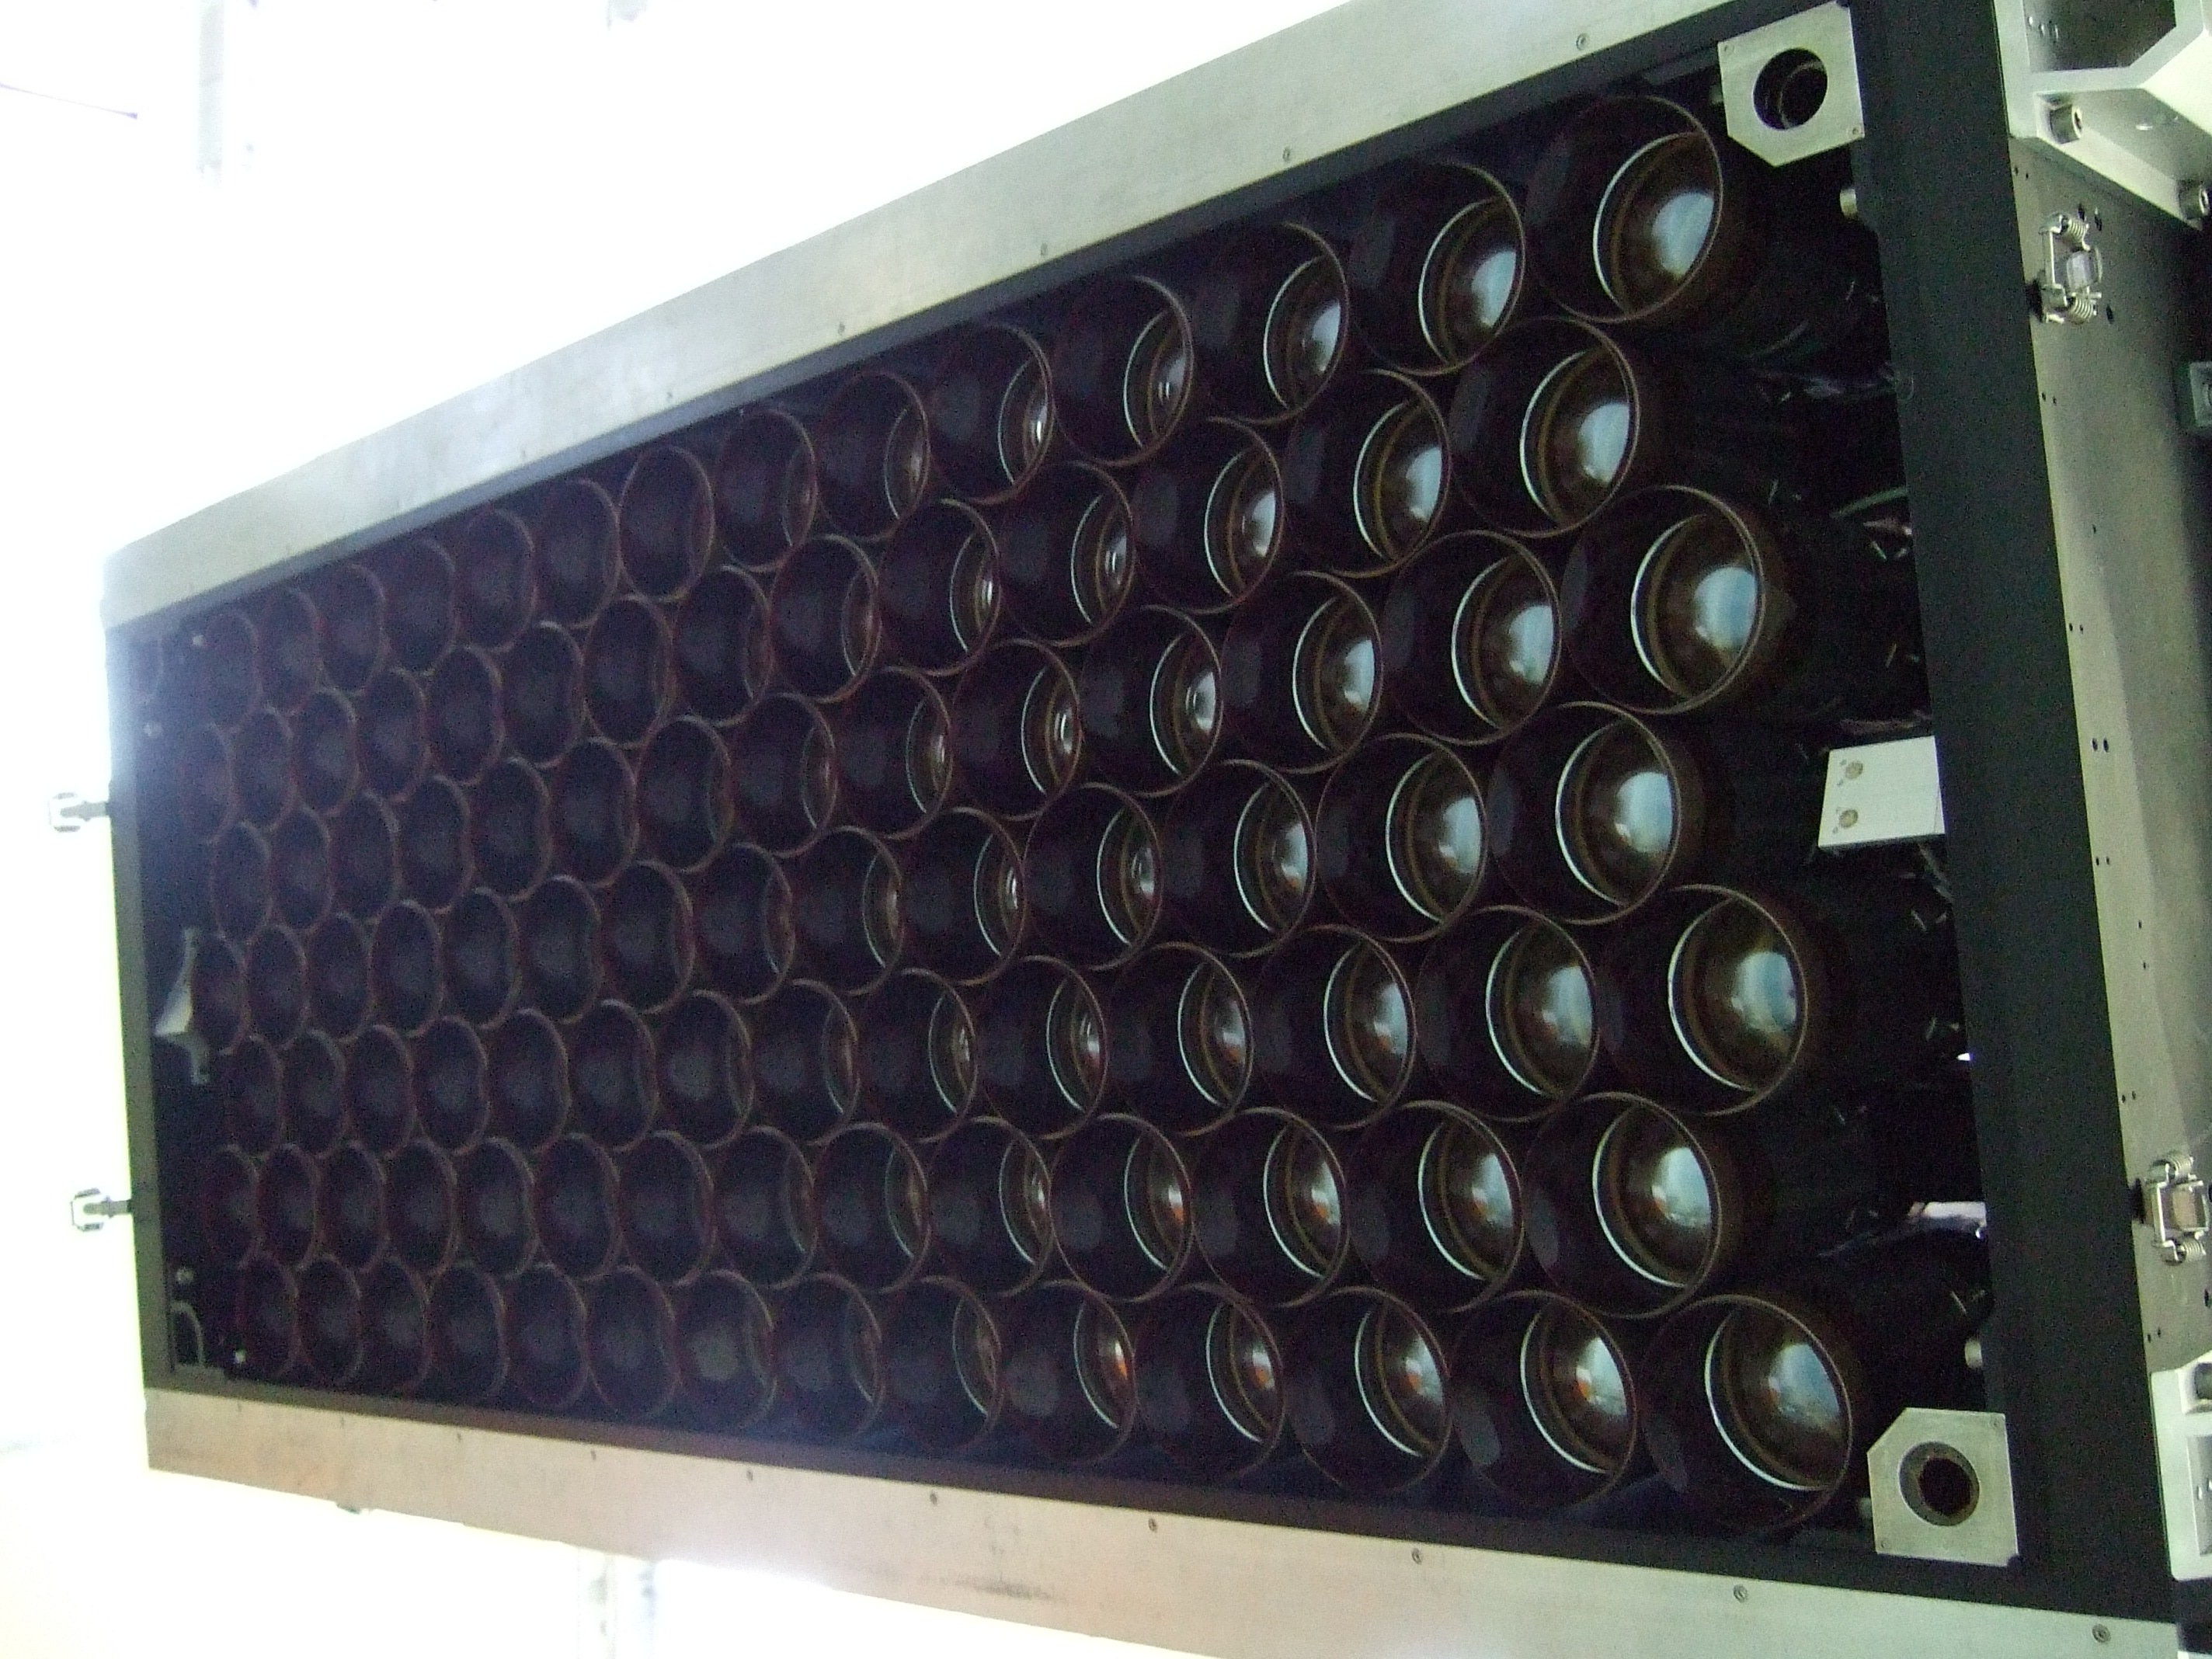
\includegraphics[width=0.5\columnwidth]{./Chapters/hpd_alignment/images/RICH1_Upper_box_134.jpg}
		\caption{Upper HPD grid in RICH 1}
		\label{fig: RICH 1: upper grid}
	\end{center}
\end{figure}

\begin{figure}
	\begin{minipage}[b]{0.45\linewidth}
		\centering
			\includegraphics[height=4cm, width=6cm]{$HOME/Dropbox/LHCb/detector/RICH/images/HPD_schematic2.png}
			\caption{HPD schematic}
			\label{fig: HPD schematic}
	\end{minipage}
	\hspace{0.5cm}
	\begin{minipage}[b]{0.45\linewidth}
		\centering
		\includegraphics[height=4cm]{$HOME/Dropbox/LHCb/detector/RICH/images/HPD_photo.jpg}
		\caption{photo of a HPD}
		\label{fig:HPD_photo}
	\end{minipage}
\end{figure}

The total accumulation of pixel signals over the course of a run can be visualised on a two dimensional plot called a hit map (or image summary fig \ref{example_HPD_image_summaries}). Due to the circular shape of the quartz window the hit map is circular in shape. An image centre is determined by fitting a circle to the boundary of the hit map and taking the central position. The accuracy in the position of the image centre is an important property of the HPD since any translation of the image centre affects the accuracy in the position of the photon, Cherenkov angle and particle identification. 

\begin{figure}
	\begin{center}
		\includegraphics[width=13cm]{$HOME/Dropbox/LHCb/detector/RICH/images/HPD_image_summaries.png}
		\caption{Example HPD hit maps for HPDs 001, 002 and 092 for run 80168. The z-axis corresponds to the number of hits registered by a pixel, the x and y axes correspond to the pixel position on the silicon chip}
		% comment: Either change the naming convention of the HPDs to match U half / D half notation and include image of layout of include image of numbered naming convention
		\label{example_HPD_image_summaries}
	\end{center}
\end{figure}

Observations of the image centre show that its position does not necessarily line up with the centre of the silicon chip, this effect is accounted for by an alignment process which reflects the displacement of the image centre from the silicon chip centre in the detector description of the LHCb detector. In addition, during the course of operation, shifts in the position of the image centre for individual HPDs have been consistently observed. These shifts can be as much as $2\,\mathrm{mm}$ (Fig \ref{fig: shift_distance}) between consecutive runs. This phenomenon was further confirmed during and investigation carried out in laboratory tests performed at the end of 2009 using HPDs removed from the LHCb detector for which shifts has been most noticeably observed. The low levels of mechanical stress, scale of the shifts (Fig \ref{fig: 2010 displacement}) and rigidity of the HPD fixings suggest the image shifts are not due to physical movement of the HPD components, but are instead the result of disturbances to the electric fields due to build up of charge on HPD components over the duration of operation. Additionally shifts were shown to be present across both magnetic field configurations and when the magnet was off suggesting this effect was not an artefact of the magnet.

In addition to the alignment of the HPD image centres the performance of the RICH detector is also dependent on the alignment of its other components. In particular the alignment of the mirrors which reflect the Cherenkov radiation onto the HPD plane and the Magnetic distortion monitoring system (MDCS) which corrects distortion effects to the HPDs due to the magnetic field from the LHCb magnet. These alignment procedures are intimately entangled such that changes in any of the alignment procedures will affect the other. Since improvements in the individual alignment systems are constantly ongoing in parallel it can be difficult to disentangle how the effect of changes in the individual alignment systems affects the RICH system as a whole. 

The work presented here builds on alignment techniques performed previously for the data collected in 2010. The main changes were to carry out the alignment on a run by run basis. For the data taking period of 2010 the HPD image centres were calculated by averaging over the whole year. Improvements were also made to the general stability and accuracy of the fit. At the time of writing the current alignment software produces improvements $\sim7\%$ in RICH1 and RICH2 (section \ref{chap: application of correction factors}) compared to the 2010 alignment techniques.

\begin{figure}
	\begin{center}
		\caption{Image centre x,y displacement and shifts for 2010 tagged consecutive runs ranging from 68179 - 80168}
		\label{fig: 2010 displacement}
		\begin{subfigure}[b]{\textwidth}%[x-displacement]
		{
			\begin{center}
				\includegraphics[width=.6\columnwidth]{/afs/cern.ch/user/d/dvoong/analysis/rich/HPDs/image_fitting/displacement_between_conseq_runs/scripts/x_displacement.png}
			\end{center}
			\caption{Displacement in x}
			\label{fig: x_displacement}
		}
		\end{subfigure}
		\begin{subfigure}[b]{\textwidth}
		{	
			\begin{center}
				\includegraphics[width=.6\columnwidth]{/afs/cern.ch/user/d/dvoong/analysis/rich/HPDs/image_fitting/displacement_between_conseq_runs/scripts/y_displacement.png}
			\end{center}
			\caption{Displacement in y}
			\label{fig: y_displacement}
		}
		\end{subfigure}
		\begin{subfigure}[b]{\textwidth}
		{
			\begin{center}
				\includegraphics[width=.6\columnwidth]{/afs/cern.ch/user/d/dvoong/analysis/rich/HPDs/image_fitting/displacement_between_conseq_runs/scripts/shift_distance.png}
			\end{center}
			\caption{Distance}
			\label{fig: shift_distance}
		}
		\end{subfigure}
	\end{center}
\end{figure}

The shifting of images was first noticed in the middle of 2009 most noticeably in a HPD located around the outer corner (HPD: A7 13) of the the A-side HPD plane (Fig \ref{fig: RICH2_HPD_plane_layout}). The RICH2 HPD intervention in October 2009 was used as an opportunity to extract the HPD to investigate image shifts in a laboratory environment. 

The set up for the laboratory tests were chosen so that the conditions were as similar as possible to the conditions in the LHCb detector. Tests were performed over time periods varying from 48 to 450 hours using an LED light source. Figure \ref{fig: november lab test} shows the results from a 48 hour period test, Figure \ref{fig: thierry row} [\ref{fig: thierry col}] shows the variation in the row [column] position of the image centre and figure \ref{fig: thierry radius} shows the variation in the radius of the circle used to fit the HPD hit map. In January 2010 the tests were repeated over a 450 hour period to investigate whether the shifts exhibited oscillatory behaviour, results are shown in figure \ref{fig: january lab test}, no significant repeating behaviour was observed.

\begin{figure}
	\begin{subfigure}[b]{\textwidth}
		\begin{center}
			\includegraphics[width=0.7\columnwidth]{$HOME/Dropbox/LHCb/detector/RICH/HPDs/alignment/thierry_stuff/november_lab_tests/pngs/row_position.png}
			\caption{image centre row position, note: lab test were performed with HPD in Alice mode meaning a greater number of effective pixels on the chip (8 Alice pixels to 1 LHCb pixel (0.5mm))}
			\label{fig: thierry row}
		\end{center}
	\end{subfigure}
	\begin{subfigure}[b]{\textwidth}
	{
		\begin{center}
			\includegraphics[width=0.7\columnwidth]{$HOME/Dropbox/LHCb/detector/RICH/HPDs/alignment/thierry_stuff/november_lab_tests/pngs/column_position.png}
			\caption{image centre column position}
			\label{fig: thierry col}
		\end{center}
	}
	\end{subfigure}
	\begin{subfigure}[b]{\textwidth}
	{
		\begin{center}
			\includegraphics[width=0.7\columnwidth]{$HOME/Dropbox/LHCb/detector/RICH/HPDs/alignment/thierry_stuff/november_lab_tests/pngs/radius.png}
			\caption{image radius}
			\label{fig: thierry radius}
		\end{center}
	}
	\end{subfigure}
	\caption{HPD A7 13 image shift lab test results over a period of four days}
	\label{fig: november lab test}
\end{figure}

\begin{figure}
	\includegraphics[width=\columnwidth]{$HOME/Dropbox/PhD/service_work/HPD_alignment/internal_note/images/january_lab_test.png}
	\caption{HPD image centre shift laboratory tests in January 2010. HPDs image shifts were monitored over a 450 hour period}
	\label{fig: january lab test}
\end{figure}
